{% -*- mode: LaTeX; TeX-PDF-mode: t; TeX-master: "manual"; -*-
}


\chapter{The \ei Toolkit Architecture}
\label{ch:architecture}

In this chapter we describe the overall design of \ei, in particular
we define its different components, their corresponding requirements
and responsibilities, and how they communicate in order to accomplish
the objectives described in Section~\ref{sec:intro:objectives}.
%
Note that the description of each \ei component is kept general in
this chapter, however, in some cases we give partial specifications to
convey the underlying ideas.
%
In chapters~\ref{ch:server}-\ref{ch:eiol}, we suggest such complete
specifications, and corresponding implementations, for each component.




\section{The Overall Architecture of \ei}
\label{ch:architecture:overallarch}

In this section we describe the overall design of \ei, which is driven
by the objectives we have stated in
Section~\ref{sec:intro:objectives}.
%
One of the most important objectives is~\objref{commonenvtrans}, which
aims at reducing the effort of integrating a tool in a common
environment, namely, it aims at achieving a situation where a tool can
be installed once, and then appears automatically in all available
environments.
%
This objective leads us to an architecture with two abstract
components:
%
\begin{enumerate}[(i)]
\item the first abstract component represents an entity where tools
  can be installed; and
\item the second abstract component represents clients (e.g.,
  development environments) that can communicate with the previous
  component to consult the list of installed tools, to execute a tool,
  etc.
\end{enumerate}
%
This abstraction leads us to a client-server architecture as depicted
in Figure~\ref{fig:eiarch}, where the \emph{server side} represents
the first abstract component, and the \emph{client side} represents
the second abstract component.

\begin{figure}[t]
\hrule\smallskip
\begin{center}
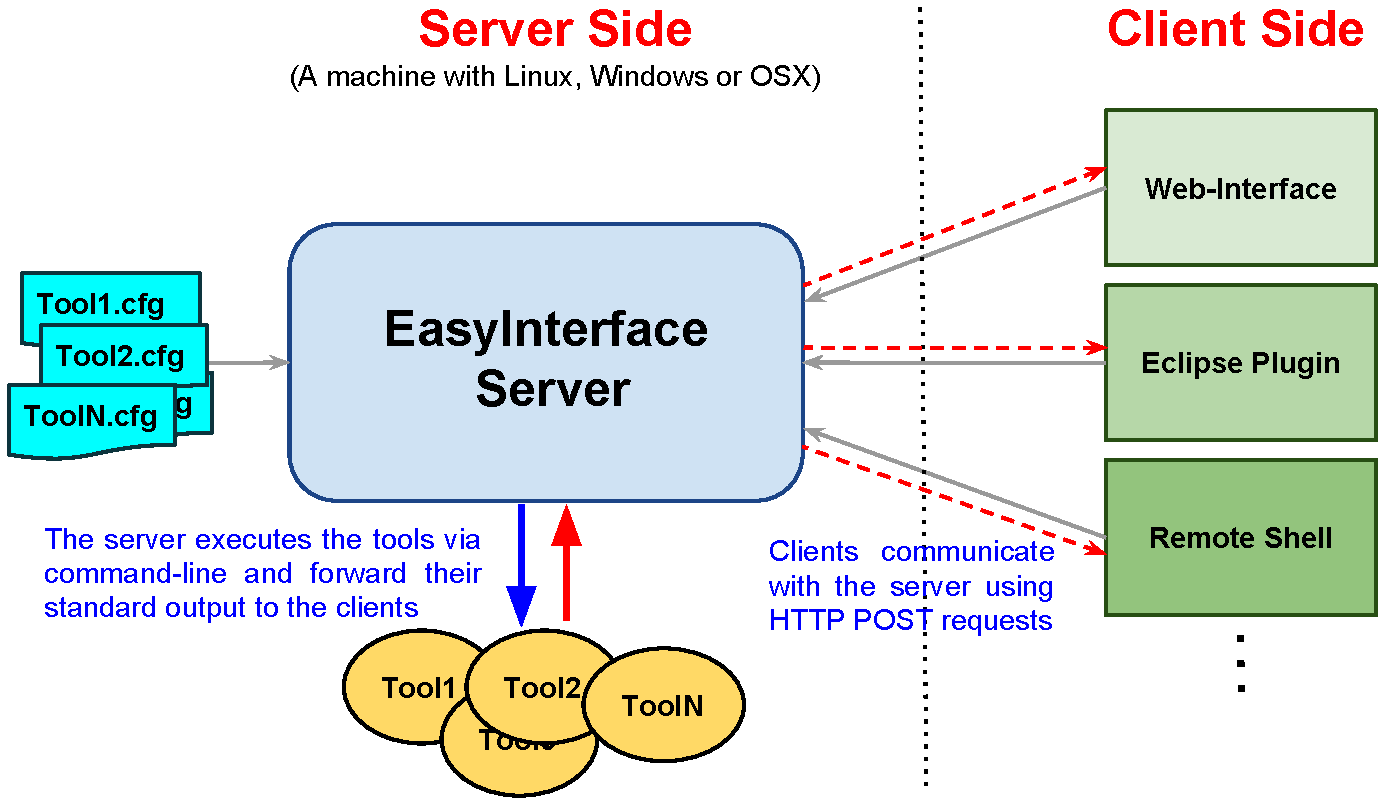
\includegraphics[width=1\textwidth]{fig/ei.pdf}
\end{center}
\caption{The Architecture of the \ei Toolkit}
\label{fig:eiarch}
\hrule
\end{figure}

%
The \emph{server side} is intended to be a machine with several tools
(the circles \texttt{Tool1}, \texttt{Tool2}, etc., in
Figure~\ref{fig:eiarch}) that can be executed from a command-line, and
their output goes to the standard output (recall that our objectives
are restricted to such tools -- see
Section~\ref{sec:intro:objectives}). These are the tools that we want
to make available for the outside world, i.e., execute them as
services on the internet.
%
The \emph{client side} includes several clients that make it easy, to
a user, to communicate with the server side to execute a tool,
etc. Clients can be simple, e.g., a program that sends a very specific
request, or more sophisticated development environments such as the
web-based one that is included in Objective~\objref{commonenv}.
%
Note that although Figure~\ref{fig:eiarch} includes only one server
component, the overall setting should allow several ones, and clients
should be configurable to connect to one or more servers.

The rest of this chapter is organized as follows. In
Section~\ref{sec:architecture:server} we explain the details of the
server side; in Section~\ref{sec:architecture:client} we explain the
details of the client side, and finally, in
Section~\ref{sec:architecture:eiol}, we explain how tools can produce
output that is shown graphically in the client side (see Objective
\objref{outputlang}).
%

\section{The Server Side}
\label{sec:architecture:server}

The problem that we want to solve at the server side can be summarized
as follows:
%
\begin{quote}
  Provide a uniform way for remotely accessing locally installed tools
  as services, such that installing new tools and accessing them is
  straightforward.
\end{quote}
%
However, this problem encapsulates different issues. In what follows,
we address these issues and draw general guidelines to corresponding
design problems. These guidelines are then used in
Chapter~\ref{ch:server} when developing the specifications of the \ei
server.

\subsection{Installing a New Tool}

Developers (of research prototype tools) should be able to make their
tools available on the server in a straightforward way, in terms of
simple configuration files (\texttt{Tool1.cfg}, \texttt{Tool2.cfg},
etc., in Figure~\ref{fig:eiarch}).
%
The only information they should provide is how the tool can be
executed from a command-line, and which parameters it takes.
%
Information about the parameters is crucial as clients will use it to
ask users to select the desired values, etc.
%
The following XML snippet suggests a format for a tool configuration
(that we actually adapt and extend in Chapter~\ref{ch:server}):

\medskip
\begin{lstlisting}
<app id="myapp">
  ...
  <execinfo>
    <cmdlineapp>(*/path-to/myapp.sh*) _ei_files _ei_parameters</cmdlineapp>
  </execinfo>
  <parameters prefix = "-" check="true">
    <selectone name="c">
      <option value="1" />
      <option value="2" />
    </selectone>
    ...
  </parameters>
</app>
\end{lstlisting}

\medskip
\noindent
This XML defines a tool that has a unique identifier \lst{myapp},
which is used to refer to this tool later.  The important parts in
this XML are the command-line tag \lst{cmdlineapp}, and the parameters
tag \lst{parameters}, that we explain next.

The content of the \lst{cmdlineapp} tag is a template that describes
how to execute the tool from a command-line. Here \lst{_ei_files} and
\lst{_ei_parameters} are \emph{template parameters} that should be
replaced, by the server, with appropriate values when receiving a
request to execute the corresponding tool.
%
As expected, \lst{_ei_files} should be replaced by a list of file
names that the client passes to the tool to process, and
\lst{_ei_parameters} by a list of parameters that the client passes to
the tool.
%
The idea of using command-line templates is very convenient, because
any information that the server wants to pass to a tool can be encoded
in such a template, and, moreover, the template can indicate which
information a tool is interested in.
%
For example, if the server maintains sessions for the different
connected clients, and the tool is interested in this information, it
can use a corresponding template parameter \lst{_ei_sessionid}.


%
The content of the \lst{parameters} tag includes a list of parameters
that are accepted by the tool. For example, in the above snippet,
there is a parameter called ``\texttt{c}'' that can take one of the
values $1$ or $2$.  
%
The \lst{prefix} attribute can be used to indicate how the parameter
is translated when passed in the command-line, e.g., one tool might
require it as \lst{-c} and another as \lst{--c}. The \lst{check}
attribute indicates if the server should check the validity of the
provided values for the different parameters, and if they are not
valid to reject the client's request.  Support for different kinds of
parameters should be provided, e.g., one value out of many, several
values out of many, Boolean parameters (i.e., either they appear or
not), free text, etc.
%

To summarize, the work-flow of the server when receiving a request to
execute a tool, with some values for the parameters, is as follows: it
replaces the template parameters with corresponding values; it
executes the corresponding command-line; and finally forwards back the
output to the client.
%
Apart from this work-flow, we can think of the following variants:
%
\begin{enumerate}[\upshape(\itshape i\upshape)]
%
\item in some tools, generating the output might take long time, and
  thus we want to disconnect the connection with the client and
  provide a key that can be used to fetch the (partial) output when it
  is ready; and
%
\item in some tools, the generated output is very large or even not in
  a text format, and thus it is convenient to provide the client with
  a link through which this output can be fetched instead of sending
  it immediately.
\end{enumerate}
%
The server should provide a mechanism for supporting such variants.

\subsection{Communicating with the Server}

Clients should be able to communicate with the server using the HTTP
POST protocol~\cite{rfc2616}. The advantage of using this protocol is that
one can build the \ei server on top of an HTTP server, and thus take
advantage of the underlying machinery for serving clients
concurrently.
%
In addition, if one is not interested in building the \ei server on
top of an HTTP server, there are numerous libraries for HTTP POST
communication that one can use (this is true for the client side as
well).

Apart from HTTP POST, the content of the actual request should also be
in a standard structured format, e.g., JSON~\cite{json}, to facilitate
their processing both at the server and client sides. For example, the
following snippet suggests a format for such requests:

\medskip
\begin{lstlisting}
{
  (*command: "execute",*)
  (*app\_id: "myapp",*)
  (*parameters:*) {
     (*c: ["1"],*)
     (*...*)
  },
  (*...*)
}
\end{lstlisting} 

\medskip
\noindent
This request indicates that we want to execute the tool identified by
\lst{myapp}, passing it some parameters as indicated in the
\lst{$\mbox{parameters}$} field, etc.
%
The \lst{$\mbox{command}$} field should support, apart from executing a
tool, other services, e.g., fetching the list of available tools,
depending on the services that are provided by the server (according
to the needs defined in the next sections).

\subsection{Example Sets}

Research prototype tools typically come with a default set of examples
from which the user can start. 
%
The server side should provide a mechanism that allows developers to
specify such sets of examples, and allows clients to fetch them as
well.
%
Specifying such a sets can be done, for example, using an XML
structure that represent a directory, where each entity that
represents a file has a URL to its actual content as well. 
%
In addition, URLs to public repositories such as GitHub should be
supported.

\subsection{Security Issues}

There are different security issues~\cite{apachesecurity} that should be considered in the
server side, among them are the following:
%
\begin{itemize}
%
\item It should be guaranteed that the client cannot manipulate the
  server, and make it execute a local program that is not supposed to
  be executed. The use of command-line templates opens a door for such
  attacks, and thus before executing the resulting command-line the
  server should guarantee that it actually executes the desired
  program and nothing else.
%
\item The server must provide a way to control the resources that can
  be consumed by a tool once it is executed, e.g., maximum cputime.
\end{itemize}
%
The server side should explicitly address the above issues, both at the
specification and implementation levels.


\section{The Client Side}
\label{sec:architecture:client}

\begin{figure}[t]
\hrule\smallskip
\begin{center}
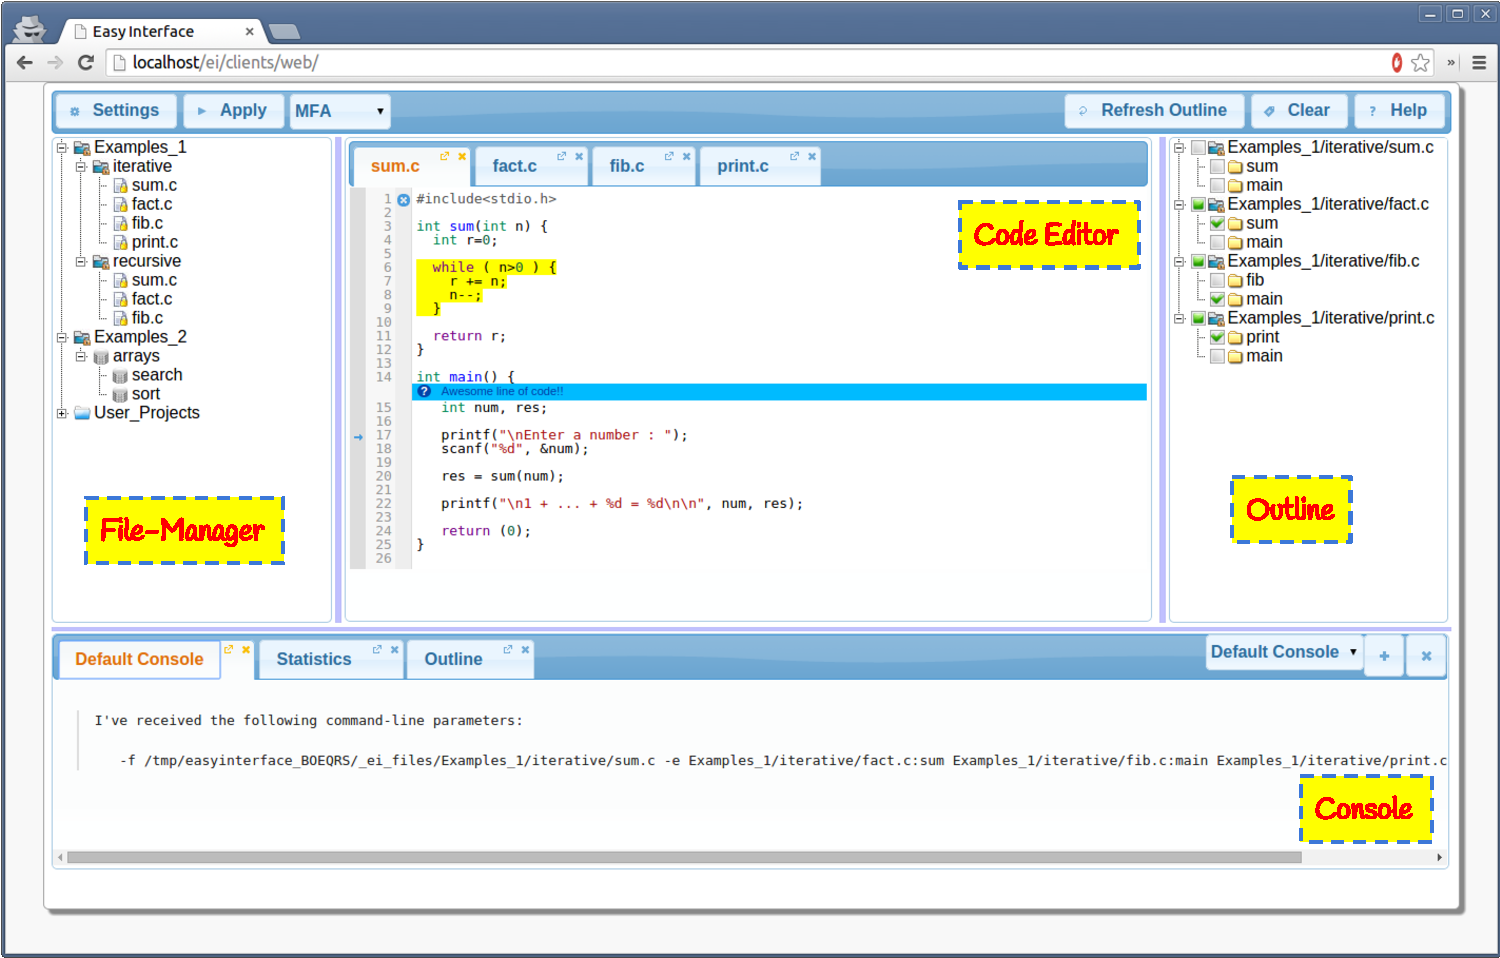
\includegraphics[width=1\textwidth]{fig/webclient.pdf}
\end{center}
\caption{\ei client example}
\label{fig:arch:client}
\hrule
\end{figure}


Although it is now relatively easy to execute tools on the server
side, as services, users would not be willing to send requests in the
above format in order to execute a tool on their own input. Thus, our
aim is to simplify this process further by providing graphical user
interfaces that:
%
\begin{enumerate}[\upshape(\itshape i\upshape)]
%
\item connect to \ei servers and ask for the list of available tools;
%
\item allow the user to select a tool to execute and set the values of
  the corresponding parameters;
%
\item generate a corresponding request and send it to the
  corresponding \ei server; and
%
\item show the returned output to the user.
\end{enumerate}
%
The \ei toolkit should provide at least one such client which is in
addition web-based, as depicted in Figure~\ref{fig:arch:client} (it is
screenshot of the actual \ei web-client -- see
Chapter~\ref{ch:clients}).
%
This client should have the following components with some associated
functionalists:
%
\begin{enumerate}[\upshape(\itshape i\upshape)]
%
\item \texttt{Code Editor}: an area were programs can be edited. This
  should support editing different programming languages easily, and
  support features such as \emph{search and replace} and \emph{syntax
    highlighting};
%
\item \texttt{File Manager}: an area that allows accessing different
  sets of examples, and also creating new programs. In addition, it
  should provide a mechanism to save and load programs, e.g., via
  GitHub repositories;
%
\item \texttt{Outline}: an area where the different elements of the
  edited programs, such as class and method names, are shown. It
  should be configurable to allow generating the outline for different
  programming languages; and
%
\item \texttt{Console}: an area where the output of a tool can be
  printed.
%
\end{enumerate}
%
In addition, this environment should include a settings section were
the parameters of the different tools (that are shown graphically) can
be set. The web-client should be configurable to include specific sets
of tools and examples, from one or more \ei servers.

%
Note that, by default, the output of a tool should be shown in the
\texttt{Console} area, unless it uses the \ei output language (see
next Section) in which case it should pass through a corresponding
interpreter to convert it to graphical widgets. Thus, such an
interpreter is expected to be an essential part of this environment.


\section{The Text-Based GUI Output Language}
\label{sec:architecture:eiol}

Since sophisticated clients that provide a development environment,
such as the web-client, are GUI based developing environments, the \ei
toolkit is required to provide tools with an easy way to view their
output as widgets in the corresponding environment (see Objective
\objref{outputlang}). This should be done in a generic way, i.e., it
should take effect in all such environments, without changing the tool
to produce specific output for each one. Thus, an output language that
abstracts away from the specific environment must be developed, and
preferably it should be text-based and does not require any knowledge
on WEB or GUI programming.
%
As a possible suggestion, the following is a snippet of such output:

\medskip
\begin{lstlisting}
<highlightlines dest="/Examples_1/iterative/sum.s"> 
  <lines> <line from="5" to="10"/> </lines>
</highlightlines>
\end{lstlisting}
%

\medskip
\noindent
This indicates that lines 5--10 of the file
\texttt{/Examples\_1/iterative/sum.s} (which is opened in the editor)
should be highlighted. This language should also provide commands that
model interaction with the user such as:

\medskip
\begin{lstlisting}
<oncodelineclick dest="/Examples_1/iterative/sum.c" outclass="info" >
  <lines><line from="17" /></lines>
  <eicommands>
    <dialogbox boxtitle="Hey!"> 
      <content format="text">
       (* Click on the marker again to close this window *)
      </content>
    </dialogbox>
  </eicommands>
</oncodelineclick>
\end{lstlisting}

\medskip
\noindent
This indicates that when clicking on line $17$, a dialog-box with a
corresponding message should be opened.
%
The language should support commands according to the needs of the
tools to which we restrict ourselves (see
Section~\ref{sec:intro:objectives}), and should be easily extensible
to meet the needs of new tools in the future.
